%\newpage
\chapter{Dentature con Profilo Cicloidale
}\label{ruotecy}
\section{Una Propriet\`a Notevole della Cicloide}

\begin{figure}[hbt]
\centering
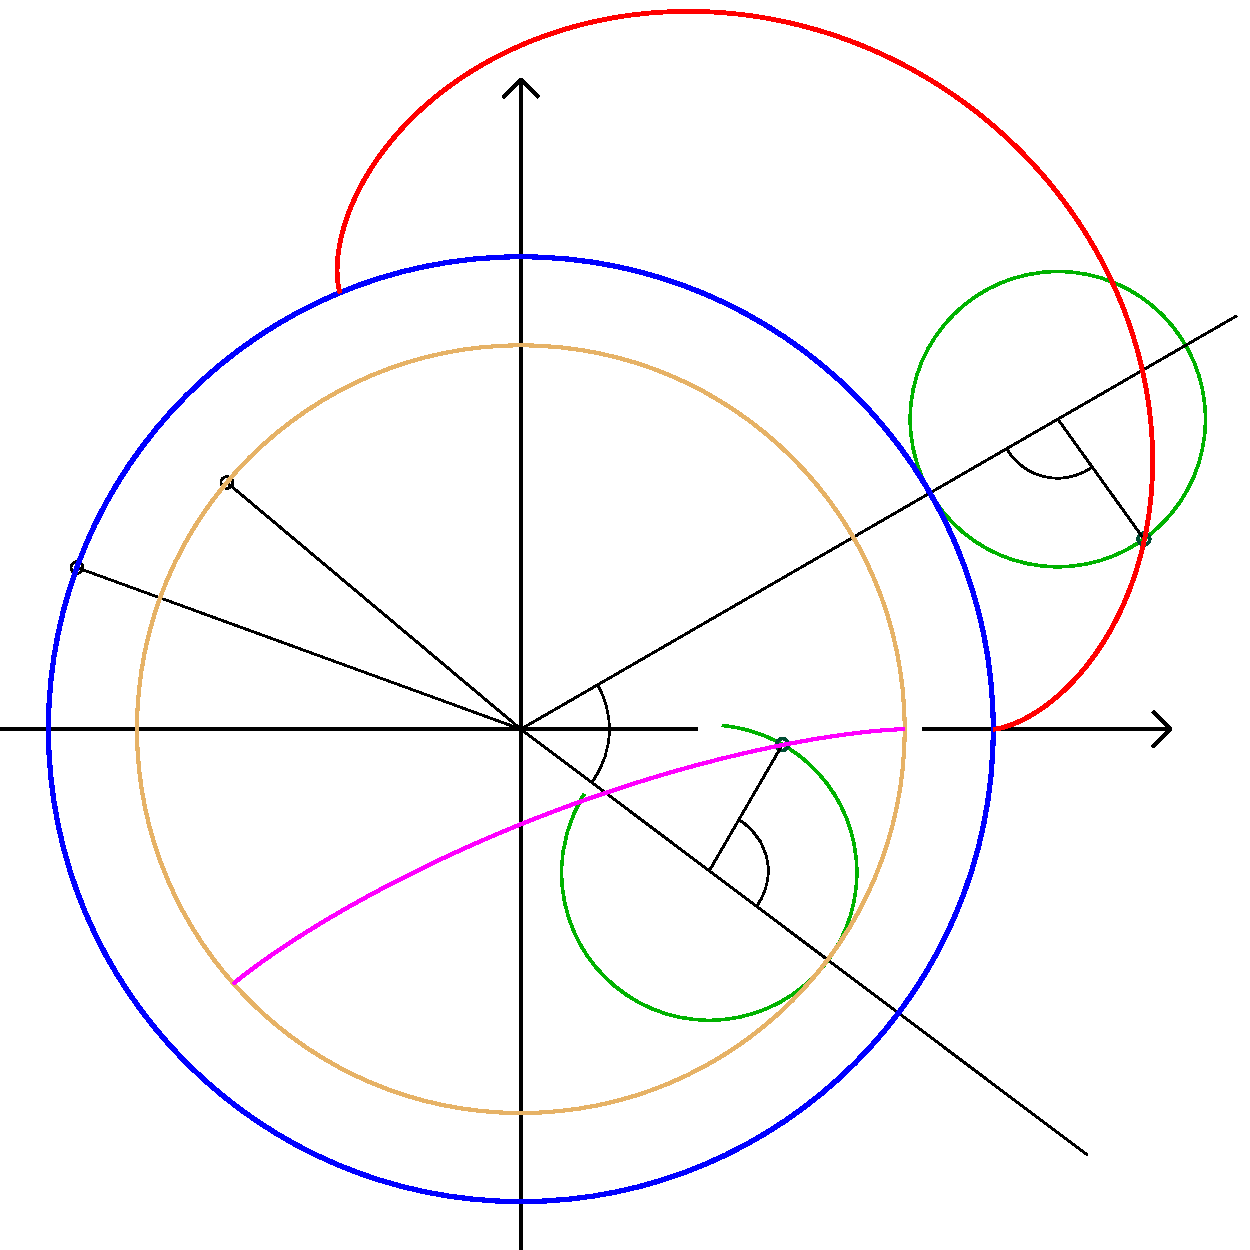
\includegraphics[width=.8\textwidth]{part3/ruote/FIG/ruote/epiipo.pdf}
\begin{picture}(0,0)(200,0)
\scriptsize{
\put(16,265){$y$}
\put(165,175){$r_r$}
\put(148,173){$\alpha$}
\put(174,161){$p_e$}
\put(-65,156){$r_1$}
\put(-33,173){$r_2$}
\put(87,93){$\alpha$}
\put(74,107){$r_r$}
\put(52,125){$t$}
\put(51,111){$\tau$}
\put(90,123){$p_i$}
\put(17,112){$O$}
\put(170,110){$x$}
}
\end{picture}
      \caption{\em Epicicloide (rosso) e ipocicloide (indaco); le circonferenze
in verde, epiciclo e ipociclo,
svolgono, rotolando, un angolo di $2\pi$.}
 \label{fig:epiipo}
\end{figure}

\noindent La curve rappresentate in figura \ref{fig:epiipo} 
di colore rosso e indaco si chiamano
rispettivamente {\em epicicloide}\index{epicicloide}
e {\em ipocicloide}\index{ipocicloide} delle circonferenze di raggio $r_1$
e $r_2$, di colori blu e arancione.
La {\em cicloide}\index{cicloide}
pu\`o essere considerata come il caso limite di queste due curve qualora la
circonferenza, sulla quale rotola l'{\em epiciclo}\index{epiciclo},
sia di raggio infinito.
L'epicicloide, rappresentata in rosso,
si ottiene facendo rotolare senza strisciamento la circonferenza verde, che
si chiama epiciclo, oppure rolletta, o anche rotella,
di raggio $r_r$ all'esterno della circonferenza di
raggio $r_1$ (colore blu) e tenendo traccia delle posizioni via via raggiunte
da un punto di tale rolletta, individuato col nome $p_e$.
Lo stesso vale per l'ipocicloide (in indaco), con la differenza che la
rolletta, ancora
di raggio $r_r$, rotola all'interno della circonferenza di raggio $r_2$
e di colore arancione: in questo caso
il punto di cui si tiene traccia si chiama $p_i$.
Abbiamo scelto di rappresentare in figura \ref{fig:epiipo} la porzione delle
due curve che si ottiene tramite  il rotolamento delle due rollette lungo
un tratto di lunghezza pari a quella della loro circonferenza.
Abbiamo altres\`i assunto arbitrariamente che ipociclo ed epiciclo abbiano
lo stesso raggio $r_r$ perch\'e, soltanto in questo caso, epicicloide e
ipocicloide saranno dotate di una interessante propriet\`a, utile nella
Meccanica delle Macchine.
\noindent Al fine di descrivere l'epicicloide tramite equazioni
parametriche, scegliamo come parametro l'angolo $t$. Le coordinate $x(t)$ e
$y(t)$ del generico punto $p_e$ si ricavano quindi tramite semplici proiezioni
\begin{equation}
\begin{cases}
{x_e}\left(t\right)=\left(r_1+r_r\right)\cos\left(t\right) +
r_r\cos\left(\pi - t - \alpha\right) \\
{y_e}\left(t\right)=\left(r_1+r_r\right)\sin\left(t\right)-
r_r\sin\left(\pi -t -\alpha\right) \,.
\end{cases}
\end{equation}
\noindent Tenendo poi conto che l'angolo $\alpha$ si pu\`o esprimere
come $\alpha = \dfrac{r_r}{r_1}t$ si ottiene
\begin{equation}
\begin{cases}
{x_e}\left(t\right)=\left(r_1+r_r\right)\cos\left(t\right) -
r_r\cos\left(\dfrac{r_1+r_r}{r_r}t\right) \\
{y_e}\left(t\right)=\left(r_1+r_r\right)\sin\left(t\right)-
r_r\sin\left(\dfrac{r_1+r_r}{r_r}t\right)\,.
\end{cases}
\label{eq:epicicloide}
\end{equation}
\noindent Nel caso dell'ipocicloide scegliamo come parametro $\tau$,
che \`e un angolo crescente in direzione opposta a $t$\footnote{
\`E usuale trovare le formule per l'ipocicloide scritte in modo analogo
a quanto si fa per l'epicicloide, cio\`e col parametro che cresce nella
direzione positiva degli angoli. In tale modo, il primo tratto della curva
occuper\`a, come avviene per l'epicicloide, il primo quadrante. L'insolita
direzione
crescente, che abbiamo scelto per $\tau$, meglio si presta alla trasformazione
di coordinate che ci
permetter\`a di mettere in relazione le due curve come profili coniugati.
}. Avremo
\begin{equation}
\begin{cases}
{x_i}\left(\tau\right)=\left(r_2-r_r\right)\cos\left(\tau\right) +
r_r\cos\left(\alpha- \tau\right) \\
{y_i}\left(\tau\right)=-\left(r_2-r_r\right)\sin\left(\tau\right)+
r_r\sin\left(\alpha -\tau\right) \,,
\end{cases}
\end{equation}
\noindent quindi
\begin{equation}
\begin{cases}
{x_i}\left(\tau\right)=\left(r_2-r_r\right)\cos\left(\tau\right) +
r_r\cos\left(\dfrac{r_2-r_r}{r_r}\tau\right) \\
{y_i}\left(\tau\right)=-\left(r_2-r_r\right)\sin\left(\tau\right)+
r_r\sin\left(\dfrac{r_2-r_r}{r_r}\tau\right)\,.
\end{cases}
\label{eq:ipocicloide}
\end{equation}
\noindent Desideriamo ora mostrare che queste due curve, epicicloide
e ipocicloide, costituiscono una coppia di profili coniugati quando
le circonferenze di raggi $r_1$ e $r_2$, alle quali debbono pensarsi solidali,
rotolano l'una sull'altra realizzando in tal modo 
le primitive di una coppia cinematica. Per la verit\`a, questa dimostrazione 
\`e gi\`a stata svolta, in modo rigoroso, nel capitolo che tratta le ruote
dentate e, in particolare, nel paragrafo che descrive l'ottenimento
di profili coniugati di assortimento. Tale dimostrazione
\`e riassunta dalle figure
\ref{fig:profili_coniugati_punto},
\ref{fig:profili_coniugati_punto_lagrange} e
\ref{fig:profili_coniugati_punto_euler},
che mostrano la coniugazione dei profili tracciati da un punto
trascinato da una primitiva che rotola su un qualsivoglia numero di altre
primitive.
Ma le dimostrazioni tanto generali, come quella riportata alla pagina
citata, nelle quali le curve in gioco 
sono generiche, dove
i procedimenti matematici tendono piuttosto all'astrazione,
dicevamo, tali dimostrazioni hanno sempre lasciato a chi scrive
un certo grado di insoddisfazione.
\begin{figure}[hbt]
\centering
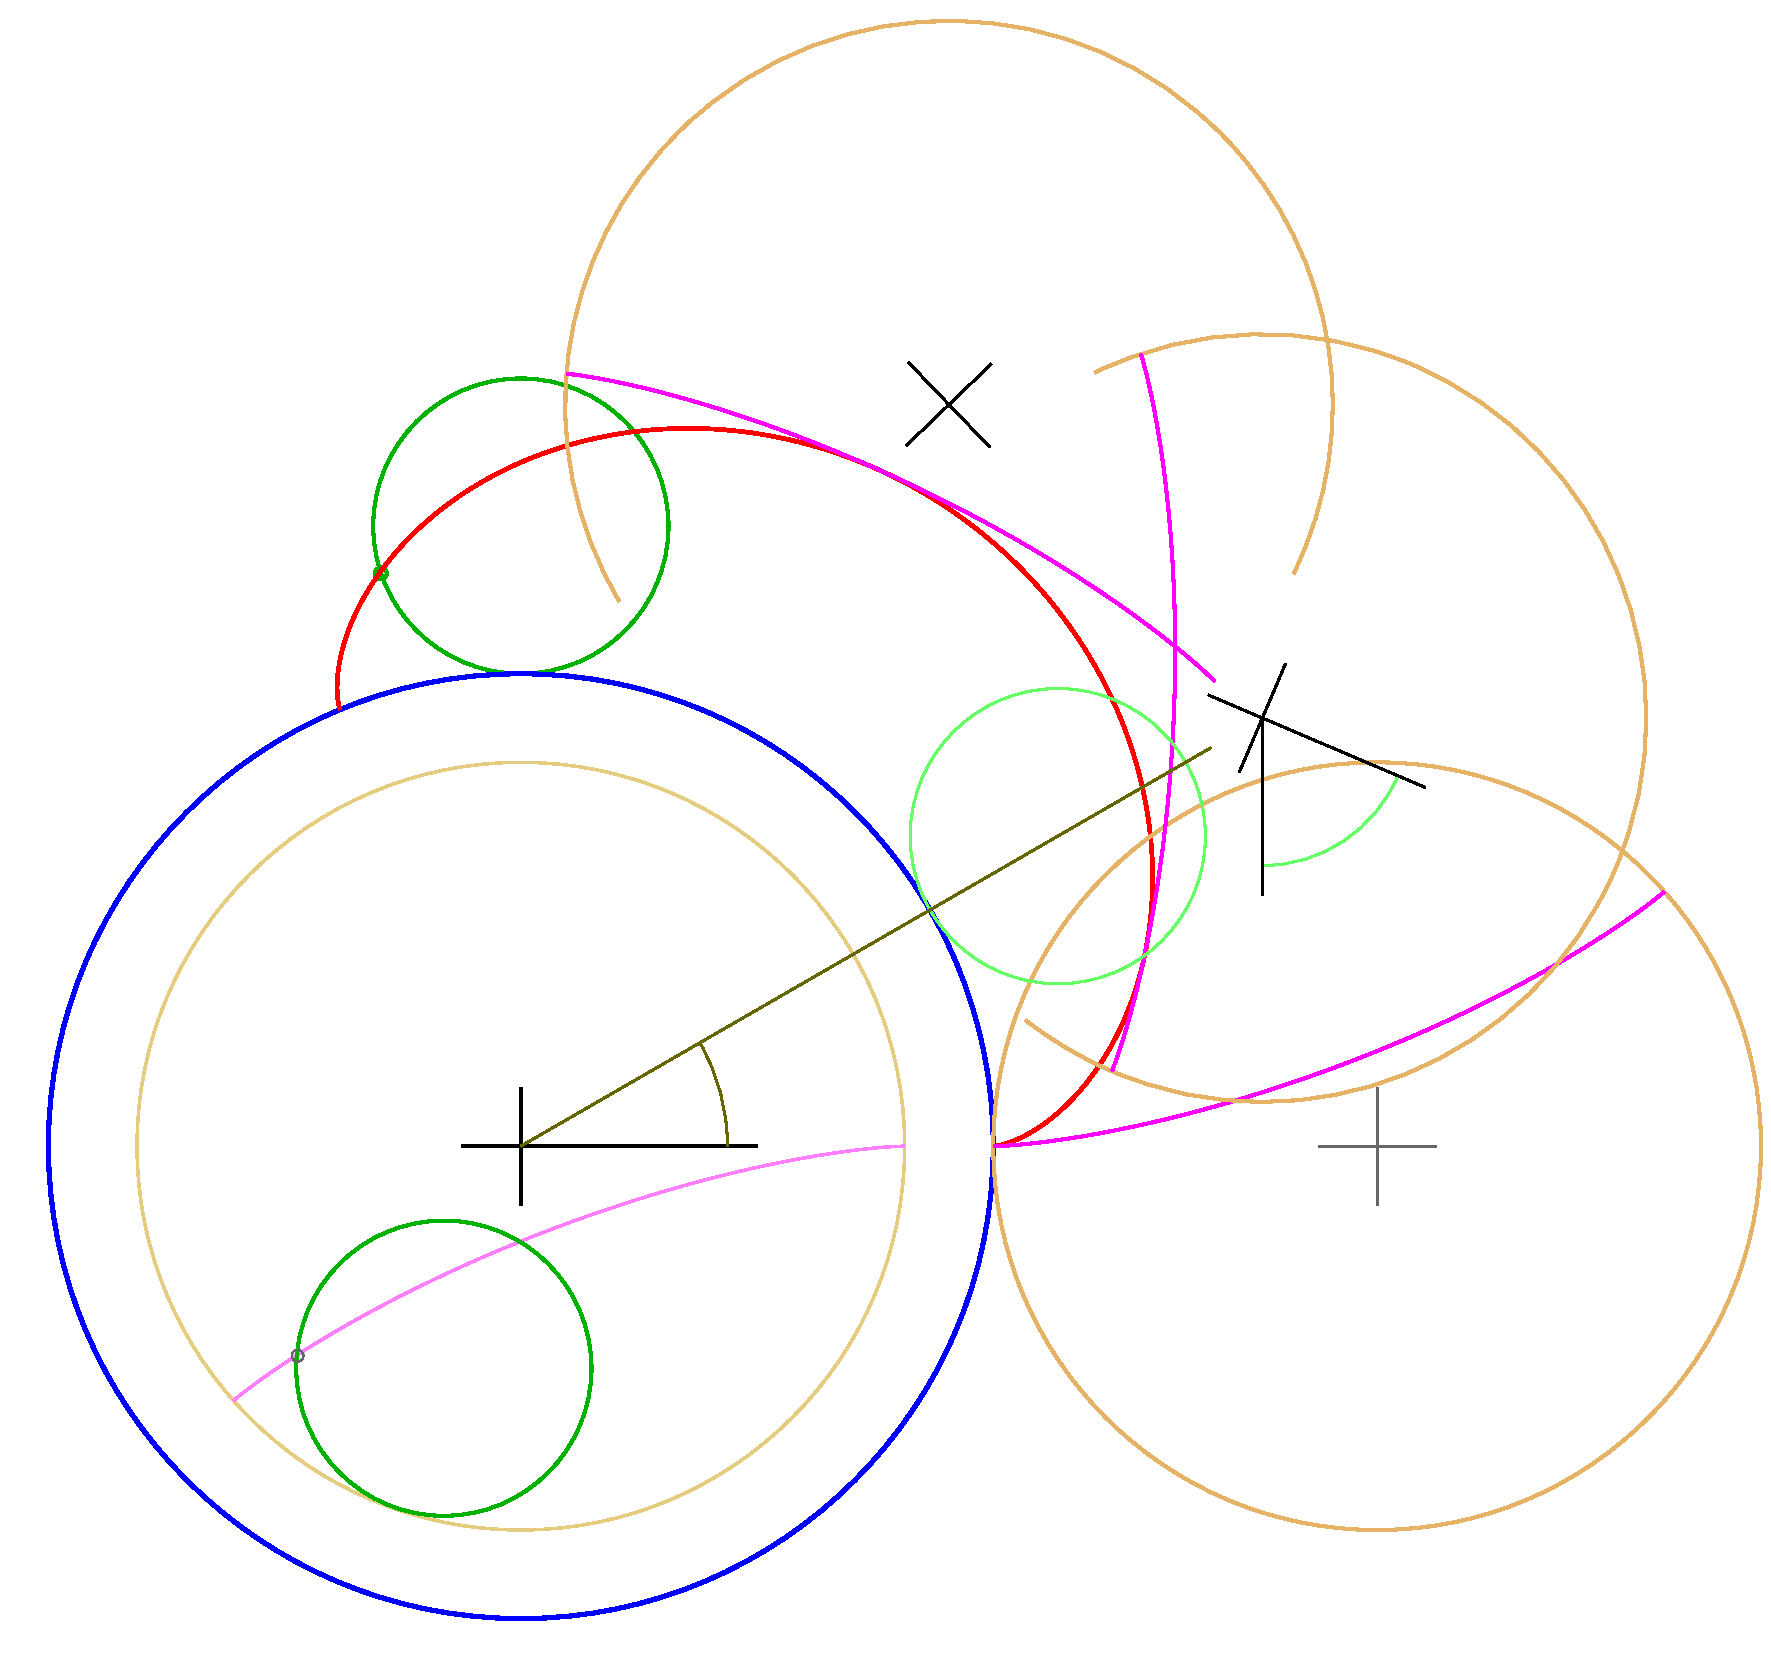
\includegraphics[width=.8\textwidth]{part3/ruote/FIG/ruote/epiipoconiugate.pdf}
\begin{picture}(0,0)(200,0)
\scriptsize{
\put(31,47){$r_2$}
\put(68,167){$t$}
\put(69,170){\rotatebox{129}{$\longrightarrow$}}
\put(144,114){$\tau$}
\put(140,106){\rotatebox{25}{$\longrightarrow$}}
\put(27,92){$t_{\scriptscriptstyle B}$}
\put(35,71){$\tau$}
\put(30,83){\rotatebox{194}{$\longrightarrow$}}
\put(-85,47){$r_1$}
\put(-18,203){$r_r$}
\put(-41,178){$p_e$}
\put(-38,49){$p_i$}
\put(-5,49){$r_r$}
\put(-18,89){$O$}
\put(120,76){$O_{\scriptscriptstyle A}$}
\put(117,155){$O_{\scriptscriptstyle B}$}
\put(57,213){$O_{\scriptscriptstyle C}$}
\put(127,130){$\phi_{\scriptscriptstyle B}$}
\put(61,83){$A$}
\put(96,112){$B$}
\put(94,104){${p_e}_{\scriptscriptstyle B}\equiv {p_i}_{\scriptscriptstyle B}$}
\put(48,199){$C$}
}
\end{picture}
      \caption{\em La ruota di raggio $r_2$ rotola su quella di raggio $r_1$ inviluppando tramite l'ipocicloide a essa solidale (indaco) la epicicloide (rosso).}
 \label{fig:epiipoconiugate}
\end{figure}
Qui riportiamo una prova
diretta, sviluppata tramite il calcolo, della coniugazione tra le due curve,
l'epicicloide e l'ipocicloide, nel caso in cui il raggio
dell'ipociclo sia uguale a quello dell'epiciclo,
suggerendo, a chi \`e gi\`a pago e convinto della dimostrazione svolta
altrove e poco interessato a questo approfondimento, di saltare
direttamente al prossimo paragrafo.
Mostreremo infatti che, scegliendo di tenere ferma
la circonferenza di raggio $r_1$, dove si svolge la epicicloide
(ma tale scelta \`e ovviamente arbitraria), e facendo rotolare 
su di essa la circonferenza di raggio $r_2$, l'ipocicloide solidale 
alla $r_2$ inviluppa proprio la epicicloide solidale alla $r_1$.
Per chiarire quanto appena affermato introduciamo la figura
\ref{fig:epiipoconiugate}, della quale la descrizione non potr\`a essere
brevissima.
Cominciamo col presentare gli attori che metteremo in campo,
dando qualche indicazione circa il ruolo che essi svolgeranno.
La circonferenza di raggio $r_1$ e centro in $O$ (di colore blu) ospita la porzione di
epicicloide (di colore rosso) svolta dalla rolletta di raggio $r_r$ quando,
rotolando all'esterno della prima, percorre una lunghezza pari alla
propria circonferenza.
Il parametro $t$, dal quale dipendono le formule
\ref{eq:epicicloide}, spazier\`a quindi nell'intervallo
 $t \in[0, 2\pi r_r/r_1]$. Circonferenza blu ed epicicloide rossa saranno
ritenute fisse, aggrappate cio\`e al foglio del libro.
\noindent Una seconda circonferenza, di raggio $r_2$, reca
la porzione di ipocicloide generata da un punto dell'ipociclo
che percorre anch'esso un cammino pari alla lunghezza della propria circonferenza, quindi
il parametro $\tau$ dell'ipocicloide
assumer\`a valori compresi nell'intervallo $\tau\ \in [0, -2\pi r_r/r_2]$.
Tale circonferenza col relativo ipociclo \`e rappresentata in quattro
diverse posizioni
con centri $O$, $O_{\scriptscriptstyle A}$, $O_{\scriptscriptstyle B}$ e $O_{\scriptscriptstyle C}$.
La circonferenza di raggio $r_2$ con centro in ${O}$,
non entrando direttamente nel processo di inviluppo, viene
riportata con tratto meno marcato
insieme alla propria ipocicloide, e posizionata
nel luogo dove vale la formula \ref{eq:ipocicloide}.
Le altre circonferenze di raggio $r_2$ sono invece traslate e rotate
in modo opportuno e come vedremo invilupperanno, tramite l'ipocicloide,
l'epicicloide solidale alla $r_1$.
\noindent Chiamiamo punti
{\em omologhi} sulla epicicloide e sulla corrispondente
ipocicloide le posizioni dei punti $p_e$ e $p_i$ corrispondenti a percorsi 
della rolletta di uguale lunghezza.
Nel nostro caso avremo $r_1 t = r_r\alpha$
e $r_2 \tau= r_r\alpha$ da cui segue immediatamente il legame
tra i due parametri $\tau = \dfrac{r_1}{r_2}t$.
\noindent La posizione della ruota di raggio $r_2$ con centro in
$O_{\scriptscriptstyle A}$ si ottiene, dalla stessa di centro $O$, mediante una
rotazione di un angolo pari a $\pi$, composta con uno spostamento verso
destra pari all'interasse $i=r_1+r_2$.
Pi\`u in generale, affinch\'e la circonferenza mobile e la relativa ipocicloide
si trovino in una posizione precisa come quelle indicate 
in successione con le lettere
$B$ e $C$, sono necessari una rotazione  e uno spostamento
degli assi a cui la \ref{eq:ipocicloide} fa riferimento.
Coerentemente coi simboli gi\`a impiegati nel paragrafo dedicato
ai profili coniugati, pag. \pageref{prof_con}, scriviamo la seguente
trasformazione per i punti della ipocicloide che la conduce nella 
posizione $B$, a partire dalla posizione centrata
\begin{equation}
\begin{pmatrix} {x_i}^\star\left(\tau\right)\\{y_i}^\star\left(\tau\right) \end{pmatrix}
={\bm T}(x_{\scriptscriptstyle B}, y_{\scriptscriptstyle B}){\bm R}(\phi_{\scriptscriptstyle B} +\pi)
\begin{pmatrix} {x_i}\left(\tau\right)\\{y_i}\left(\tau\right) \end{pmatrix}\,,
 \label{eq:rot_trasl_i}
\end{equation}
\noindent avendo indicato con ${x_i}\left(\tau\right)$ e ${y_i}\left(\tau\right)$
 i punti della ipocicloide centrata in $O$, mentre con
${x_i}^\star\left(\tau\right)$ e con ${y_i}^\star\left(\tau\right)$
indichiamo le loro trasformazioni.
Una delle condizioni che deve essere soddisfatta,
affinch\'e le due curve risultino coniugate, risiede 
nella coincidenza, nella posizione $B$, dei punti delle due curve.
In altri termini, deve essere verificato che
\begin{equation}
\begin{pmatrix} {x_e}\left(t_{\scriptscriptstyle B}\right)\\{y_e}\left(t_{\scriptscriptstyle B}\right) \end{pmatrix}=
\begin{pmatrix} {x_i}^\star\left(\tau_{\scriptscriptstyle B}\right)\\{y_i}^\star\left(\tau_{\scriptscriptstyle B}\right)
\end{pmatrix}
={\bm T}(x_{\scriptscriptstyle B}, y_{\scriptscriptstyle B}){\bm R}(\phi_{\scriptscriptstyle B} +\pi)
\begin{pmatrix} {x_i}\left(\tau_{\scriptscriptstyle B}\right)\\{y_i}\left(\tau_{\scriptscriptstyle B}\right)
\end{pmatrix}\,,
 \label{eq:rot_trasl_ei}
\end{equation}
\noindent dove ${x_e}\left(t_{\scriptscriptstyle B}\right)$ e
${y_e}\left(t_{\scriptscriptstyle B}\right)$ sono le coordinate 
dell'epicicloide nel punto di interesse.
\noindent Scriviamo la
\ref{eq:rot_trasl_ei} in forma esplicita
\begin{multline}
\begin{pmatrix} {x_i}^\star\left(\tau_{\scriptscriptstyle B}\right)\\{y_i}^\star\left(\tau_{\scriptscriptstyle B}\right) \end{pmatrix} =
\begin{pmatrix} \cos(\phi_{\scriptscriptstyle B}+\pi) &-\sin(\phi_{\scriptscriptstyle B}+\pi)\\
		 \sin(\phi_{\scriptscriptstyle B}+\pi) &\cos(\phi_{\scriptscriptstyle B}+\pi) \end{pmatrix}
\begin{pmatrix} {x_i}\left(\tau_{\scriptscriptstyle B}\right)\\{y_i}\left(\tau_{\scriptscriptstyle B}\right) \end{pmatrix} + \\
+ \begin{pmatrix} (r_1+r_2)\cos(t_{\scriptscriptstyle B})\\(r_1+r_2)\sin(t_{\scriptscriptstyle B}) \end{pmatrix}\,,
\label{eq:ipocicloide_ruototraslata}
\end{multline}
\noindent nella quale la matrice, che compare
appena a destra del segno di uguaglianza, opera la rotazione piana di un angolo 
pari a $\phi_{\scriptscriptstyle B}+\pi$.
\noindent Mostriamo ora che i punti
${p_e}_{\scriptscriptstyle B}$ e ${p_i}_{\scriptscriptstyle B}$ coincidono
a valle della roto-traslazione,
fatto peraltro evidente dalla figura composta per via numerica.
Utilizziamo a questo scopo la \ref{eq:ipocicloide_ruototraslata}, inserendo per
${x_i}\left(\tau{\scriptscriptstyle B}\right)$ e ${y_i}\left(\tau{\scriptscriptstyle B}\right)$
quelli forniti dalla \ref{eq:ipocicloide}, e avendo cura di sostituire, al
parametro $\tau$, il suo omologo $t$, che origina la posizione $B$.
Ponendo quindi $\tau{\scriptscriptstyle B} = {r_1\over{r_2}}t_{\scriptscriptstyle B}$ e
$\phi_{\scriptscriptstyle B}={{r_1+r_2}\over{r_2}}t_{\scriptscriptstyle B}$,
per la prima riga delle \ref{eq:ipocicloide_ruototraslata} avremo
\begin{multline}
{x_i}^\star\left(\tau_{\scriptscriptstyle B}\right)=
[-\left(r_2-r_r\right)\cos\left({r_1\over{r_2}}t_{\scriptscriptstyle B}\right)\cos\left({{r_1+r_2}\over{r_2}}t_{\scriptscriptstyle B}\right) + \\ -
r_r\cos\left({{r_2-r_r}\over{r_r}}{r_1\over{r_2}}t_{\scriptscriptstyle B}\right)\cos\left({{r_1+r_2}\over{r_2}}t_{\scriptscriptstyle B}\right) + \\ -
\left(r_2-r_r\right)\sin\left({r_1\over{r_2}}t_{\scriptscriptstyle B}\right)\sin\left({{r_1+r_2}\over{r_2}}t_{\scriptscriptstyle B}\right) + \\ +
r_r\sin\left({{r_2-r_r}\over{r_r}}{r_1\over{r_2}}t_{\scriptscriptstyle B}\right)\sin\left({{r_1+r_2}\over{r_2}}t_{\scriptscriptstyle B}\right)] + \\ +
\left(r_1+r_2\right)\cos\left(t_{\scriptscriptstyle B}\right)\,,
\label{eq:inviluppo_x}
\end{multline}
\noindent e facendo buon uso delle formule di somma per gli archi
otteniamo infine
\begin{equation}
{x_i}^\star\left(\tau_{\scriptscriptstyle B}\right)=\left(r_1+r_r\right)\cos\left(t_{\scriptscriptstyle B}\right) -
r_r\cos\left(\dfrac{r_1+r_r}{r_r}t_{\scriptscriptstyle B}\right)=
{x_e}\left(t_{\scriptscriptstyle B}\right)\,.
\label{eq:invdimostrato}
\end{equation}
\noindent Crediamo inutile riportare anche l'espressione
di ${y_i}^\star\left(\tau_{\scriptscriptstyle B}\right)$ che coincide naturalmente
con la
${y_e}\left(t_{\scriptscriptstyle B}\right)$
riportata nelle \ref{eq:epicicloide}, per $t=t_{\scriptscriptstyle B}$.
Tali espressioni per le coordinate del punto della ipocicloide
ci assicurano che
${p_i}_{\scriptscriptstyle B}\equiv{p_e}_{\scriptscriptstyle B}$,
e la coincidenza test\'e dimostrata vale naturalmente per tutti i punti
omologhi dell'epicicloide e dell'ipocicloide.
Ci\`o per\`o non \`e sufficiente per mostrare che la ipocicloide inviluppa,
durante il suo moto, la curva epicicloide:
a tale scopo occorre infatti provare che, nei punti omologhi,
anche le tangenti alle due curve coincidono, circostanza anche
questa evidente dalla figura. Le  derivate delle coordinate dell'epicicloide
risultano essere
\begin{equation}
\begin{cases}
\dfrac{{\rm d}{x_e}\left(t\right)}{{\rm d}t} = 
\left(r_1+r_r\right)
[-\sin\left(t\right) +
\sin\left(\dfrac{r_1+r_r}{r_r}t\right)] \\
\dfrac{{\rm d}{y_e}\left(t\right)}{{\rm d}t} = 
\left(r_1+r_r\right)
[\cos\left(t\right) -
\cos\left(\dfrac{r_1+r_r}{r_r}t\right)]
\end{cases}\,,
\label{eq:depicicloide}
\end{equation}
\noindent mentre quelle delle derivate dell'ipocicloide sono
\begin{equation}
\begin{cases}
\dfrac{{\rm d}{x_i}\left(\tau\right)}{{\rm d}\tau} = 
\left(r_2-r_r\right)
[-\sin\left(\tau\right) -
\sin\left(\dfrac{r_2-r_r}{r_r}\tau\right)] \\
\dfrac{{\rm d}{y_i}\left(\tau\right)}{{\rm d}\tau} = 
\left(r_2-r_r\right)
[-\cos\left(\tau\right) +
\cos\left(\dfrac{r_2-r_r}{r_r}\tau\right)]
\end{cases}\,.
\label{eq:dipocicloide}
\end{equation}

\noindent Ruotando queste ultime derivate, calcolate in $B$, dell'angolo
$\phi_{\scriptscriptstyle B}+\pi$  otteniamo
\begin{equation}
\begin{pmatrix}
\dfrac{{\rm d}{x_i}\left(\tau\right)}{{\rm d}\tau}
\\
\dfrac{{\rm d}{y_i}\left(\tau\right)}{{\rm d}\tau}
\end{pmatrix}^\star_{\scriptscriptstyle B}
 =
\begin{pmatrix} \cos(\phi + \pi) &-\sin(\phi + \pi)\\
		 \sin(\phi + \pi) &\cos(\phi + \pi) \end{pmatrix}
\begin{pmatrix}
\dfrac{{\rm d}{x_i}\left(\tau\right)}{{\rm d}\tau}
\\
\dfrac{{\rm d}{y_i}\left(\tau\right)}{{\rm d}\tau}
\end{pmatrix}_{\scriptscriptstyle B}\,,
\label{eq:derivata_ruotata}
\end{equation}
\noindent dove si pu\`o notare l'assenza del termine relativo
 alla traslazione in quanto trattandosi di trasformare delle 
differenze tra coordinate essa avrebbe effetto nullo.
Sostituendo, come si \`e fatto in precedenza,
$\tau_{\scriptscriptstyle B} = {\dfrac{r_1}{r_2}}t_{\scriptscriptstyle B}$ e
$\phi_{\scriptscriptstyle B}={\dfrac{r_1+r_2}{r_2}}t_{\scriptscriptstyle B}$
otteniamo
\begin{multline}
\dfrac{{\rm d}{x_i}\left(\tau\right)}{{\rm d}\tau}\bigr|^\star_{\scriptscriptstyle B} = 
[\left(r_2-r_r\right)\sin\left(\dfrac{r_1}{r_2}t_{\scriptscriptstyle B}\right)
\cos\left(\dfrac{r_1+r_2}{r_2}t_{\scriptscriptstyle B}\right) + \\ +
\left(r_2-r_r\right)\sin\left(\dfrac{r_1}{r_2}\dfrac{r_2-r_r}{r_r}t_{\scriptscriptstyle B}\right)
\cos\left(\dfrac{r_1+r_2}{r_2}t_{\scriptscriptstyle B}\right) + \\ -
\left(r_2-r_r\right)\cos\left(\dfrac{r_1}{r_2}t_{\scriptscriptstyle B}\right)
\sin\left(\dfrac{r_1+r_2}{r_2}t_{\scriptscriptstyle B}\right) + \\ +
\left(r_2-r_r\right)\cos\left(\dfrac{r_1}{r_2}\dfrac{r_2-r_r}{r_r}t_{\scriptscriptstyle B}\right)
\sin\left(\dfrac{r_1+r_2}{r_2}t_{\scriptscriptstyle B}\right)]\,,
\label{eq:dx_in_t}
\end{multline}
\noindent cio\`e
\begin{equation}
\dfrac{{\rm d}{x_i}\left(\tau\right)}{{\rm d}\tau}\bigr|^\star_{\scriptscriptstyle B} = 
\left(r_2+r_r\right)[-\sin\left(t_{\scriptscriptstyle B}\right) +
\sin\left(\dfrac{r_1+r_r}{r_r}t_{\scriptscriptstyle B}\right)]\,,
\label{eq:dx}
\end{equation}
\noindent mentre, ripetendo il precedente calcolo, che preferiamo non riportare
esplicitamente, per la coordinata $y$ otterremmo
\begin{equation}
\dfrac{{\rm d}{y_i}\left(\tau\right)}{{\rm d}\tau}\bigr|\star_{\scriptscriptstyle B} = 
\left(r_2+r_r\right)[\cos\left(t_{\scriptscriptstyle B}\right) -
\cos\left(\dfrac{r_1+r_r}{r_r}t_{\scriptscriptstyle B}\right)]\,.
\label{eq:dy}
\end{equation}
\noindent Le espressioni \ref{eq:dx} e \ref{eq:dy} coincidono, a meno di
un fattore moltiplicativo, con le espressioni
delle derivate dell'epicicloide \ref{eq:depicicloide} calcolate in $B$.
La differenza tra i fattori che moltiplicano le derivate
dipende dal fatto che $t$ e $\tau$ sono parametri in generale diversi tra
loro e generano quindi differenti rapporti incrementali.
Questa circostanza per\`o nulla toglie alla nostra dimostrazione, in quanto si
avr\`a
\begin{equation}
\dfrac{\dfrac{{\rm d}{x_e}\left(t\right)}{{\rm d}t}\bigr|_{\scriptscriptstyle B}}{\dfrac{{\rm d}{y_e}\left(t\right)}{{\rm d}t}\bigr|_{\scriptscriptstyle B}} =
\dfrac{\dfrac{{\rm d}{x_i}\left(\tau\right)}{{\rm d}\tau}\bigr|^\star_{\scriptscriptstyle B}}
{\dfrac{{\rm d}{y_i}\left(\tau\right)}{{\rm d}\tau}\bigr|^\star_{\scriptscriptstyle B}} \,,
\label{eq:dtot}
\end{equation}
\noindent che prova la coincidenza delle tangenti alla curva inviluppante e
al relativo inviluppo nel generico punto $B$.
Abbiamo cos\`i mostrato che, durante il rotolamento di una ruota di
raggio $r_2$ su una di raggio $r_1$, che possiamo immaginare ferma,
l'ipocicloide, trascinata dalla ruota mobile, inviluppa un tratto di epicicloide
della ruota fissa corrispondente al medesimo epiciclo.
In definitiva, pensando alle circonferenze in gioco come alle polari del moto,
i due tratti di epicicloide e ipocicloide si comporteranno come profili
coniugati essendo costantemente a contatto e possedendo la stessa
tangente\footnote{
Nessuna ipotesi riguardante i raggi delle circonferenze \`e stata messa in campo
quindi il raggio della rolletta $r_r$ potrebbe superare quello delle
circonferenze sulle quali sviluppa le cicloidi. Nel caso di
 $r_r$ di lunghezza infinita otteniamo per le due curve archi di evolvente.
}.

\section{Ruote con Denti a Profilo Cicloidale}

\noindent Dalle conclusioni del precedente paragrafo, come anche dalle
conclusioni del paragrafo \ref{prof_con}, emerge con chiarezza la possibilit\`a
di usare i profili cicloidali per modellare i fianchi dei denti di ruote,
aventi primitive circolari,
che garantiscano la trasmissione omocinetica del moto. Contrariamente 
per\`o a quanto visto per le ruote i cui denti presentano un
profilo a evolvente di cerchio,
trattando i profili cicloidali siamo costretti a dividere i profili coniugati
in due porzioni: considerando il punto di contatto tra le
primitive, una di queste si trover\`a 
dalla parte della prima ruota mentre l'altra porzione si trover\`a
dalla parte della seconda ruota. Contenendo, poi, ciascuna delle due porzioni
dei profili ora citate, due tratti distinti, un primo di epicicloide
e un secondo di ipocicloide,
il numero di spezzoni (i quali costituiranno la sagoma dei denti) da considerare sar\`a in definitiva quattro.
Ad esempio, volendo
usare una porzione della epicicloide e della ipocicloide rappresentate in
 figura \ref{fig:epiipoconiugate}, il tratto appartenente alla epicicloide
potr\`a rappresentare la sporgenza del dente sulla ruota $r_1$, 
 mentre un tratto sulla ipocicloide
costituir\`a la rientranza sulla ruota $r_2$.
Non rimane quindi altra scelta che
ripetere quanto fatto per le due primitive a ruoli invertiti: generare cio\`e
una epicicloide sulla ruota $r_2$
e una ipocicloide sulla $r_1$. Ci preme sin d'ora sottolineare
tre aspetti importanti delle ruote a profilo cicloidale,
che ci indirizzano sulla strada della loro costruzione.
La prima considerazione riguarda proprio la coniugazione
a tratti dei profili dei denti:
teste e fianchi sono tra loro coniugati, ma non lo sono i profili
nella loro interezza.
Ci\`o ci convince facilmente che l'interasse di progetto
dovr\`a essere rigidamente rispettato e che le due circonferenze primitive
potranno solo coincidere con quelle di raggi
$r_1$ e $r_2$: le relative coppie di profili coniugati si scambieranno
il testimone proprio quando il loro punto di contatto cadr\`a su queste
circonferenze.
La seconda considerazione \`e una diretta conseguenza della
prima: gli epicicli usati per ottenere le due coppie di profili possono essere
tra loro diversi, circostanza questa
che, come vedremo pi\`u avanti, semplifica la
 costruzione di queste ruote in un determinato perimetro di applicazione che
\`e quello dell'orologeria.
\`E chiaro che risulteranno ``di assortimento'' soltanto quelle ruote
aventi il medesimo passo o, ci\`o che \`e equivalente, lo stesso modulo, 
costruite mediante lo stesso epiciclo o mediante coppie di epicicli uguali
tra loro.
Da ultimo notiamo che l'inconveniente del numero minimo di
denti -- il quale
nel caso di ruote con denti a evolvente deriva dall'impossibilit\`a
di
estendere il fianco dei denti stessi oltre le circonferenze di base,
in questo caso, scegliendo opportunamente il raggio delle rollette --
non si manifesta, essendo entrambe le coppie di profili
prolungabili (entro certi limiti) a volont\`a.

\section{Proporzionamento delle Ruote Cicloidali}

\noindent Rimane valido anche per queste ruote il proporzionamento
dei denti legato al modulo della ruota stessa? Ancora, \`e necessario,
oppure utile, introdurre anche qui tale concetto?
Come sappiamo, nell'ambito della progettazione delle ruote ad evolvente, una
stretta disciplina che lega la forma dei denti, in particolare
{\em addendum} e {\em dedendum}, al modulo $m$ rende la loro progettazione
pi\`u semplice.
Si pu\`o sicuramente definire, anche nel caso di profilo cicloidale,
il modulo $m=2 r/z$, pari cio\`e, come al solito, al diametro primitivo
diviso il numero di denti.
Una volta definito tale modulo, saremmo in grado di riferire ad esso
l'{\em addendum} e il {\em dedendum} dei denti utilizzando proporzioni che si ispirino a
 quelle delle ruote a evolvente.  Ci\`o che si ottiene
in tal caso, per un ingranaggio $z_1=11$ e $z_2=60$, \`e riportato in figura
\ref{fig:1160cy}.

\begin{figure}[hbt]
     \begin{center}
     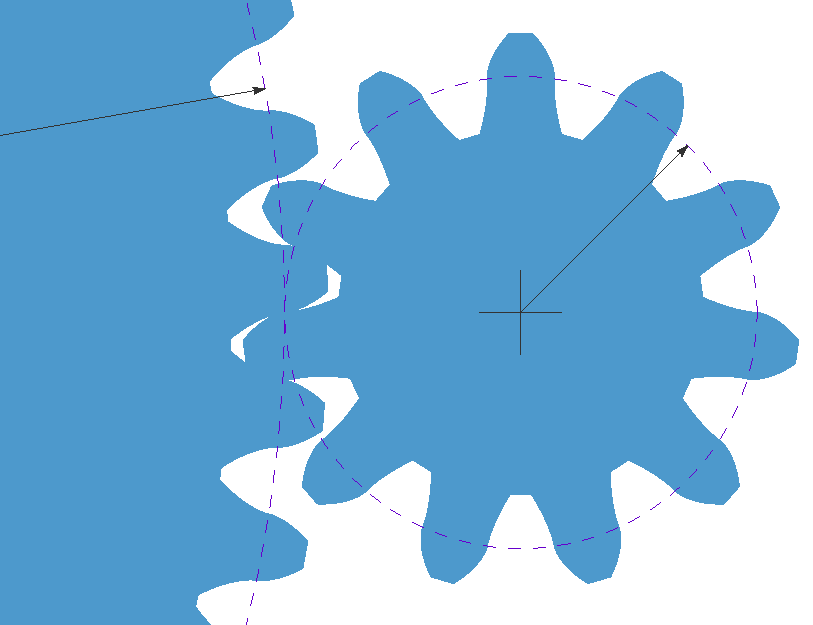
\includegraphics[width=0.9\textwidth]{part3/ruote/FIG/ruote/1160cy.pdf}
     \end{center}
\begin{picture}(0,0)(0,0)
        \scriptsize{
        \put(112,243){$r_2$}
        \put(290,207){$r_1$}
        \put(232,142){$O_1$}
}
\end{picture}
\vskip -5mm
        \caption{
\em Generico ingranaggio cicloidale con $r_1=40$,  $z_1=11$, $z_2=60$ e
raggio degli epicicli $r_i=r_e=10$.
}
     \label{fig:1160cy}
\end{figure}

\noindent La scelta dei numeri di denti, per l'ingranaggio di questa figura,
non \`e casuale: la figura
\ref{fig:1160}, che riporta un ingranaggio tra ruote a evolvente
recanti gli stessi numeri di denti, mette infatti in evidenza, sul pignone,
la problematica che si chiama sottotaglio dei denti, oppure
interferenza. Dalla figura \ref{fig:1160cy} risulta invece evidente che tale
problema non si manifesta per le ruote cicloidali, per le quali \`e
persino possibile un numero di denti pari a due.
A dire il vero per\`o, l'ingranaggio cicloidale, sopra riportato, ci convince
fino a un certo segno. Intanto, come \`e esplicitato nella didascalia,
siamo costretti a evidenziare i raggi degli epicicli utilizzati che, nel nostro
caso, a fronte di un raggio primitivo del pignone pari a $r_1=40$,
valgono $r_e=r_i=10$ (le unit\`a di misura sono qui volutamente omesse).
Il raggio unico dell'epiciclo e dell'ipociclo sulla
prima ruota equivale naturalmente a quello dell'ipociclo e dell'epiciclo
sulla seconda. Il valore di tale raggio giunge da una raccomandazione
contenuta in \cite{punzi}, la quale segnala che la proporzione ottimale tra
il raggio della rolletta e il modulo della ruota \`e $r_e=r_i=1.375 m$,
risultando cos\`i possibile
tagliare pignoni con pochi denti senza incorrere nell'indebolimento della
base dei suoi denti. In teoria, potremmo quindi affermare che tutte
 le generiche ruote disegnate in questo modo e
 aventi lo stesso modulo risulterebbero essere
``di assortimento''. Ma \`e subito chiaro che, nell'ambito di queste
dentature, la scelta
tutto sommato arbitraria dei raggi di epiciclo e ipociclo, i raggi
dei quali si adattano forzatamente ad essere rapportati al modulo della ruota,
indebolisce molto il concetto di assortimento, e con esso quello stesso
di modulo che invece, nel caso delle ruote ad evolvente, lega bens\`i il
loro numero di denti al loro diametro primitivo, ma soprattutto 
seleziona
un utensile, usando il quale si possono tagliare
ruote che risultano tutte compatibili tra loro. Quindi, modulo s\`i, ma segnatamente
in quanto passo diametrale, il quale individua, in sostanza, le dimensioni
dell'oggetto che stiamo considerando. Vedremo a breve uno {\em standard}
che riguarda la fabbricazione di ruote per orologeria, dove il concetto
di modulo non solo \`e usato ma porta con s\'e un folto numero di
relazioni tra le quantit\`a geometriche che modellano, in quell'ambito,
i denti. Ciononostante, anche in quel mondo il concetto di assortimento
\`e molto pi\`u sfumato rispetto a quello che si trova studiando le ruote ad
evolvente. Tornando all'ingranaggio di figura \ref{fig:1160cy}, chi scrive 
non \`e sicuro che il  proporzionamento di generiche ruote cicloidali si esegua
seguendo quella via. Non siamo neppure sicuri che ruote come quelle
di figura \ref{fig:1160cy} siano mai state tagliate (nel caso, ovviamente,
con fresatura di forma), e ammettiamo senza difficolt\`a  di non
averle mai viste dal vero.


\section{Interessanti Casi di Ruote Cicloidali}

L'epilogo, relativamente privo di entusiasmo, del precedente paragrafo non
deve disincentivare la nostra indagine circa le eventuali applicazioni di questi
ingranaggi, meno comuni dei loro ``cugini'' a evolvente.
Toccheremo infatti brevemente gli aspetti geometrici
di tre tipologie particolari di
ruote con denti a profilo cicloidale, ciascuno dei quali presenta
interessanti applicazioni
concrete nella tecnica. La terza, in ordine di presentazione,
di queste famiglie di ruote gode anzi
di diffusione copiosa e capillare
perch\'e riguarda gli ingranaggi presenti negli orologi.

\noindent Un primo caso peculiare di dentatura cicloidale
emerge dalla possibilit\`a che gli ipocicli siano
le stesse circonferenze primitive. Le ipocicloidi si riducono, in tal caso,
a un punto, mentre le epicicloidi saranno tracciate dai punti di una
delle due primitive che rotola sull'altra.
Generalmente, si sceglie di far seguire a un certo numero di punti della
primitiva del pignone, punti che corrisponderanno ai suoi ``denti'',
le traiettorie di epicicloide disegnate dalla circonferenza
primitiva del  pignone stesso mentre rotola
sulla circonferenza primitiva dell'altra ruota.
I punti individuati sul pignone dovrebbero, in teoria,
 seguire fisicamente i fianchi dei 
denti con profilo epicicloidale, ma essi non potrebbero
offrire che contatti singolari,
poco idonei a trasmettere forze e, in generale, inutilizzabili nelle
applicazioni tecniche. Per questo motivo, si sostituiscono
tali punti con idonee rotelle di raggio  opportuno
e, di conseguenza,  si modifica la forma del fianco cicloidale dei
denti della ruota
condotta in modo che tali fianchi siano l'inviluppo delle
rotelle stesse quando il loro centro segue l'epicicloide.
Si ottengono in questo modo
le cosiddette 
{\em ruote a lanterna}\index{ruote!a lanterna}, il cui nome deriva 
dalla particolare forma del pignone dell'ingranaggio che pu\`o ricordare
una lanterna. Un esempio di queste ruote \`e riportato in figura \ref{fig:lanterna}.
Gli ingranaggi a lanterna vengono impiegati per movimentare ruote
 condotte
di grandi diametri e possono sopportare condizioni di lavoro gravose.
Quando il raggio
della ruota condotta diventa infinito il pignone a lanterna muove
una cremagliera. In questo caso i centri delle rotelle percorrono
dei tratti di cicloide. Quest'ultima soluzione si trova in alcuni
nastri trasportatori soggetti a carichi ingenti.
\begin{figure}[t]
     \begin{center}
     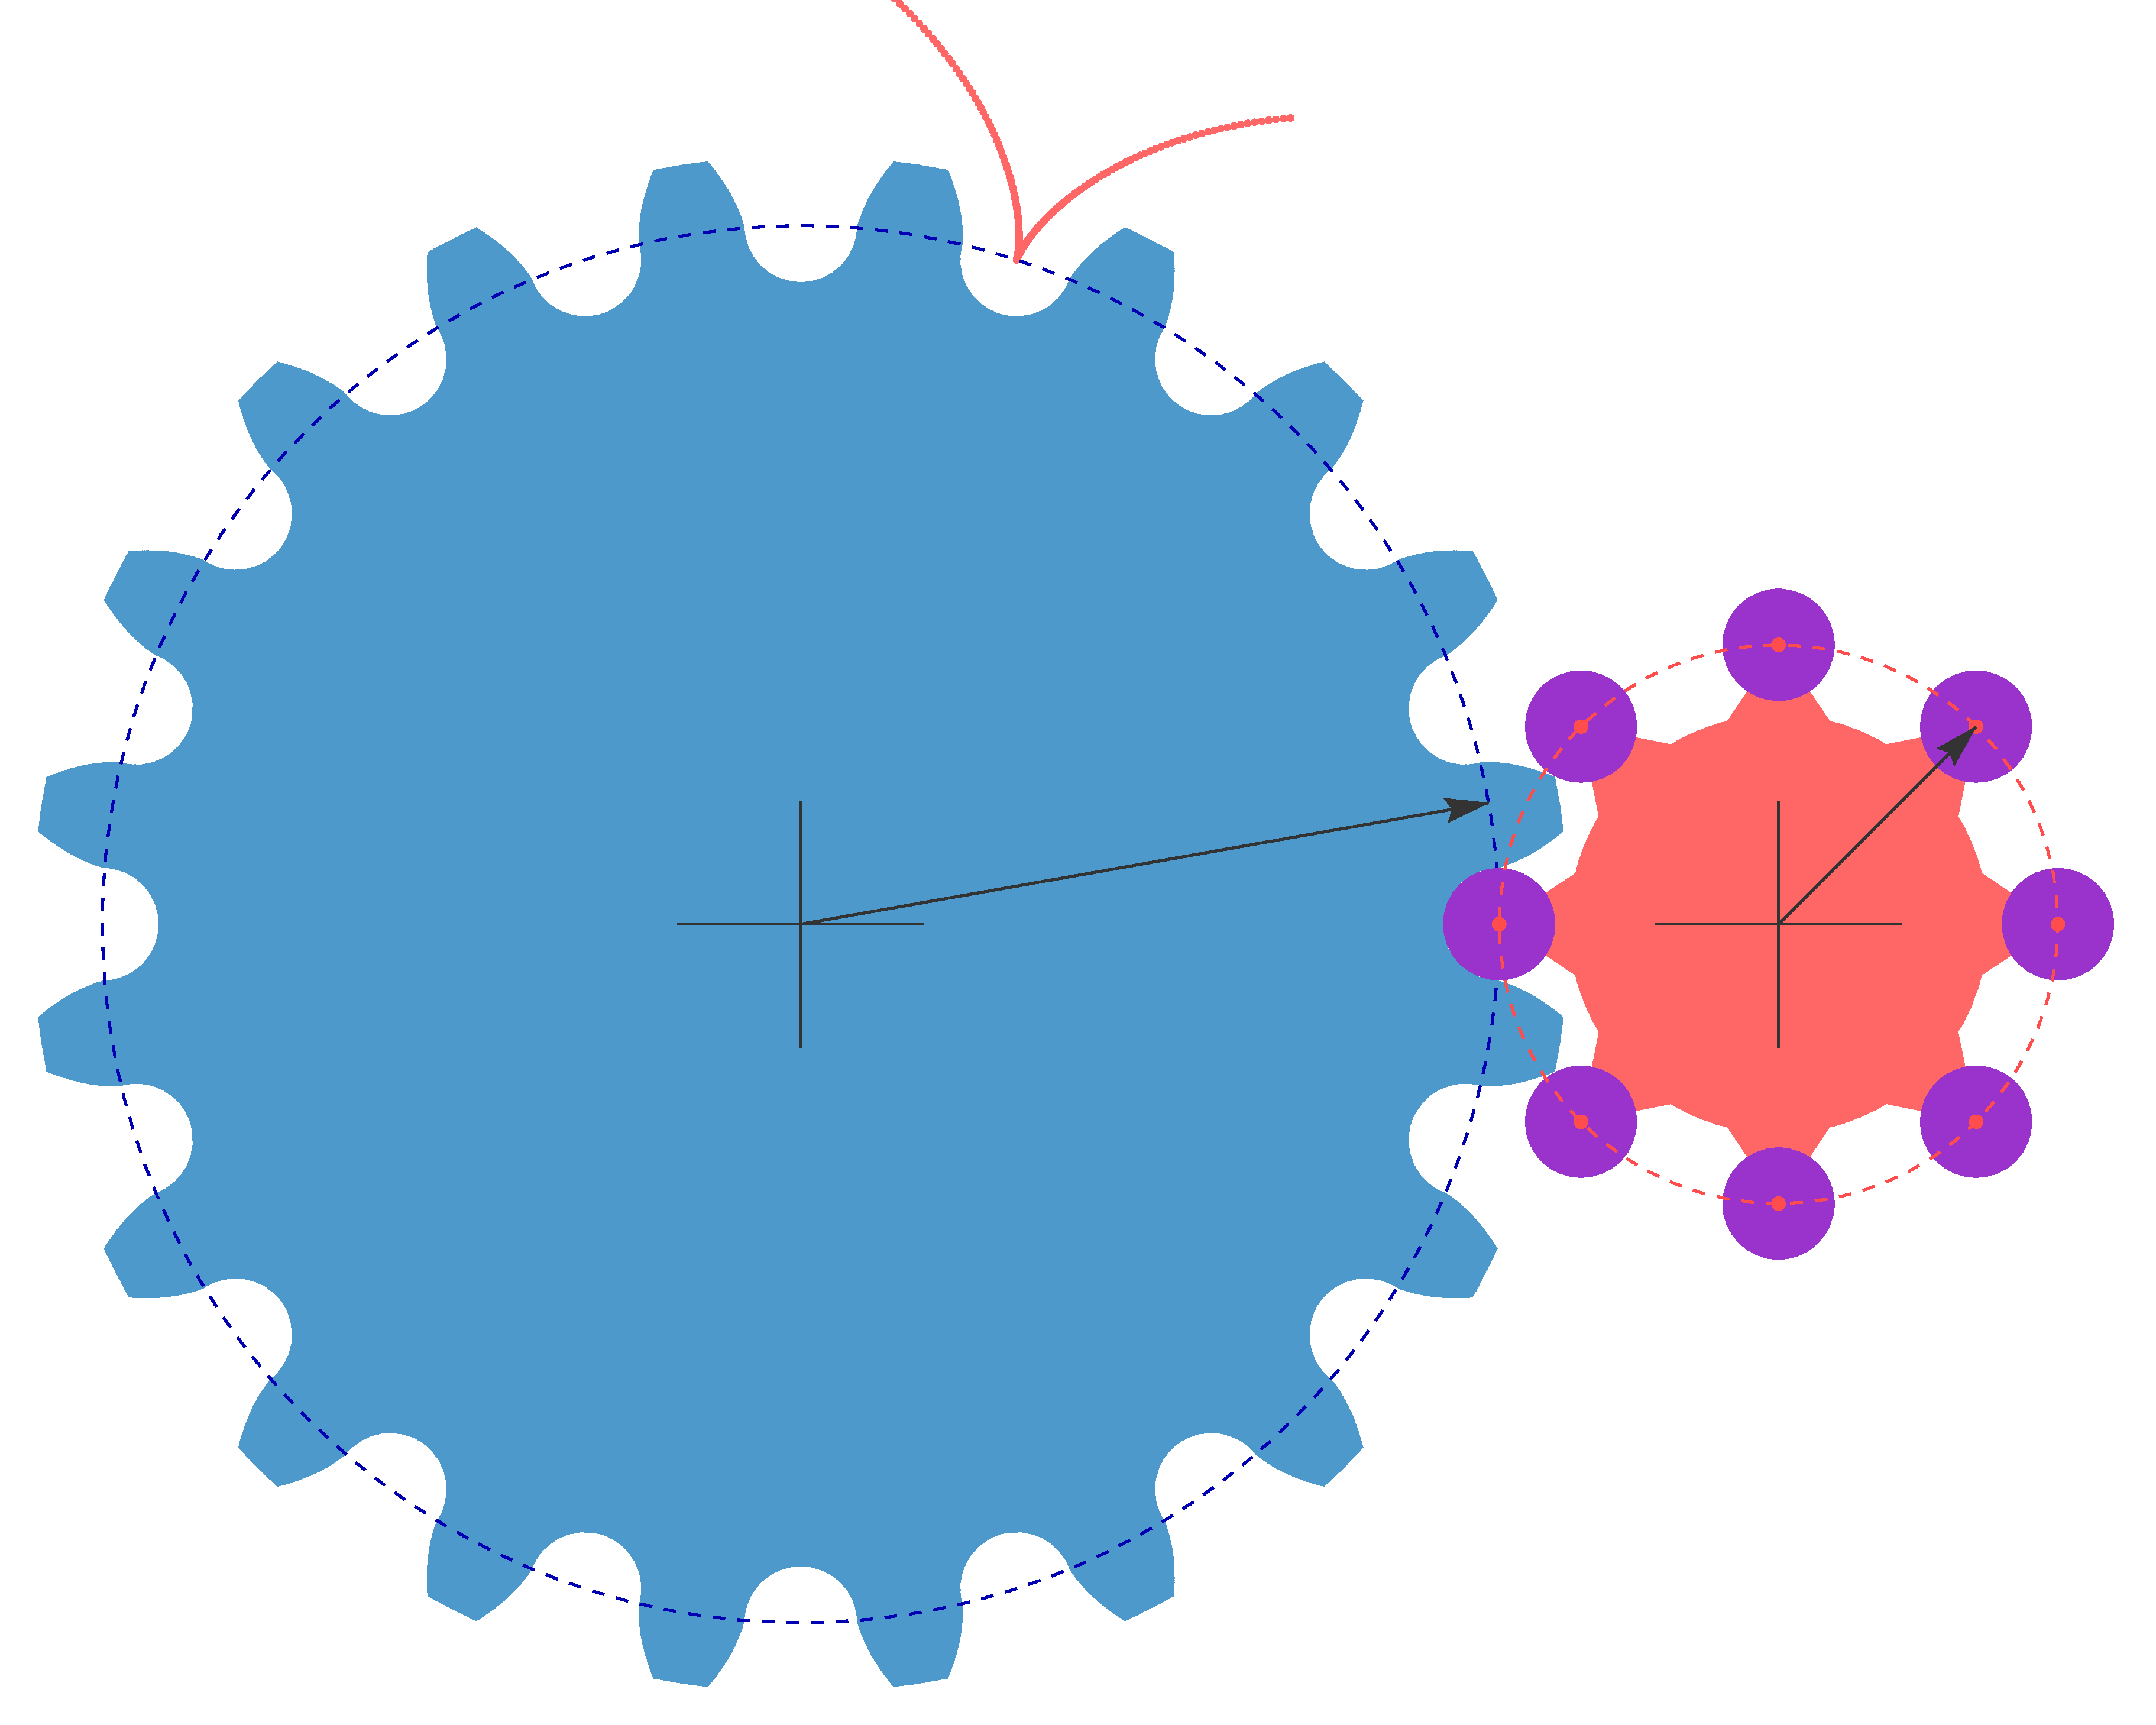
\includegraphics[width=0.9\textwidth]{part3/ruote/FIG/ruote/lanterna.pdf}
     \end{center}
\begin{picture}(0,0)(0,0)
        \scriptsize{
        \put(220,165){$r_2$}
        \put(294,165){$r_1$}
        \put(290,136){$O_1$}
        \put(127,136){$O_2$}
	\put(215,270){tratto di epicicloide, $r_e=r_1$}
}
\end{picture}
\vskip -5mm
        \caption{
\em Ruota cicloidale con pignone a lanterna, $z_1=8$, $z_2=20$.
}
     \label{fig:lanterna}
\end{figure}

\noindent Abbiamo accennato alla possibilit\`a di ottenere
ruote cicloidali con numero di denti ridottissimo.
Un particolare dispositivo atto a comprimere o pompare fluidi si
ottiene dall'ingranaggio di ruote con denti cicloidali a due o a tre 
denti.
Descriviamo il caso di ruote con due denti, che riportiamo in figura
\ref{fig:kompressor}, specificando che le proporzioni da rispettare
per ottenere tale meccanismo sono le seguenti:
$z=2$, $r_1=r_2$ e $r_e=r_i= r_1/4$.
Le ruote, disegnate mediante il proporzionamento proposto,
non sono certo in grado di trasmettere tra loro
il moto con continuit\`a. Tuttavia, qualora la loro rotazione venga garantita
da una adeguata coppia di ruote dentate esterne,
esse ingranano, da un punto di vista
puramente cinematico, correttamente.
Tali {\em ruote a lobi}\index{ruote!a lobi}, alterando periodicamente
i volumi a loro disposizione nel corpo della pompa, assicurano
fino ad un certo grado la tenuta stagna, quindi la possibilit\`a di comprimere
o di pompare i fluidi. Esistono diverse versioni commerciali di questi
dispositivi che prendono il nome di {\em pompe a lobi}\index{pompe a lobi},
quando elaborano
fluidi incomprimibile, oppure di {\em compressori volumetrici  a lobi}
quando trattano gas comprimibili.
Una nota casa automobilistica installava, fino a 
non molto tempo fa, questo tipo di compressore per sovralimentare
diversi dei suoi modelli di motore a combustione interna.
\begin{figure}[t]
     \begin{center}
     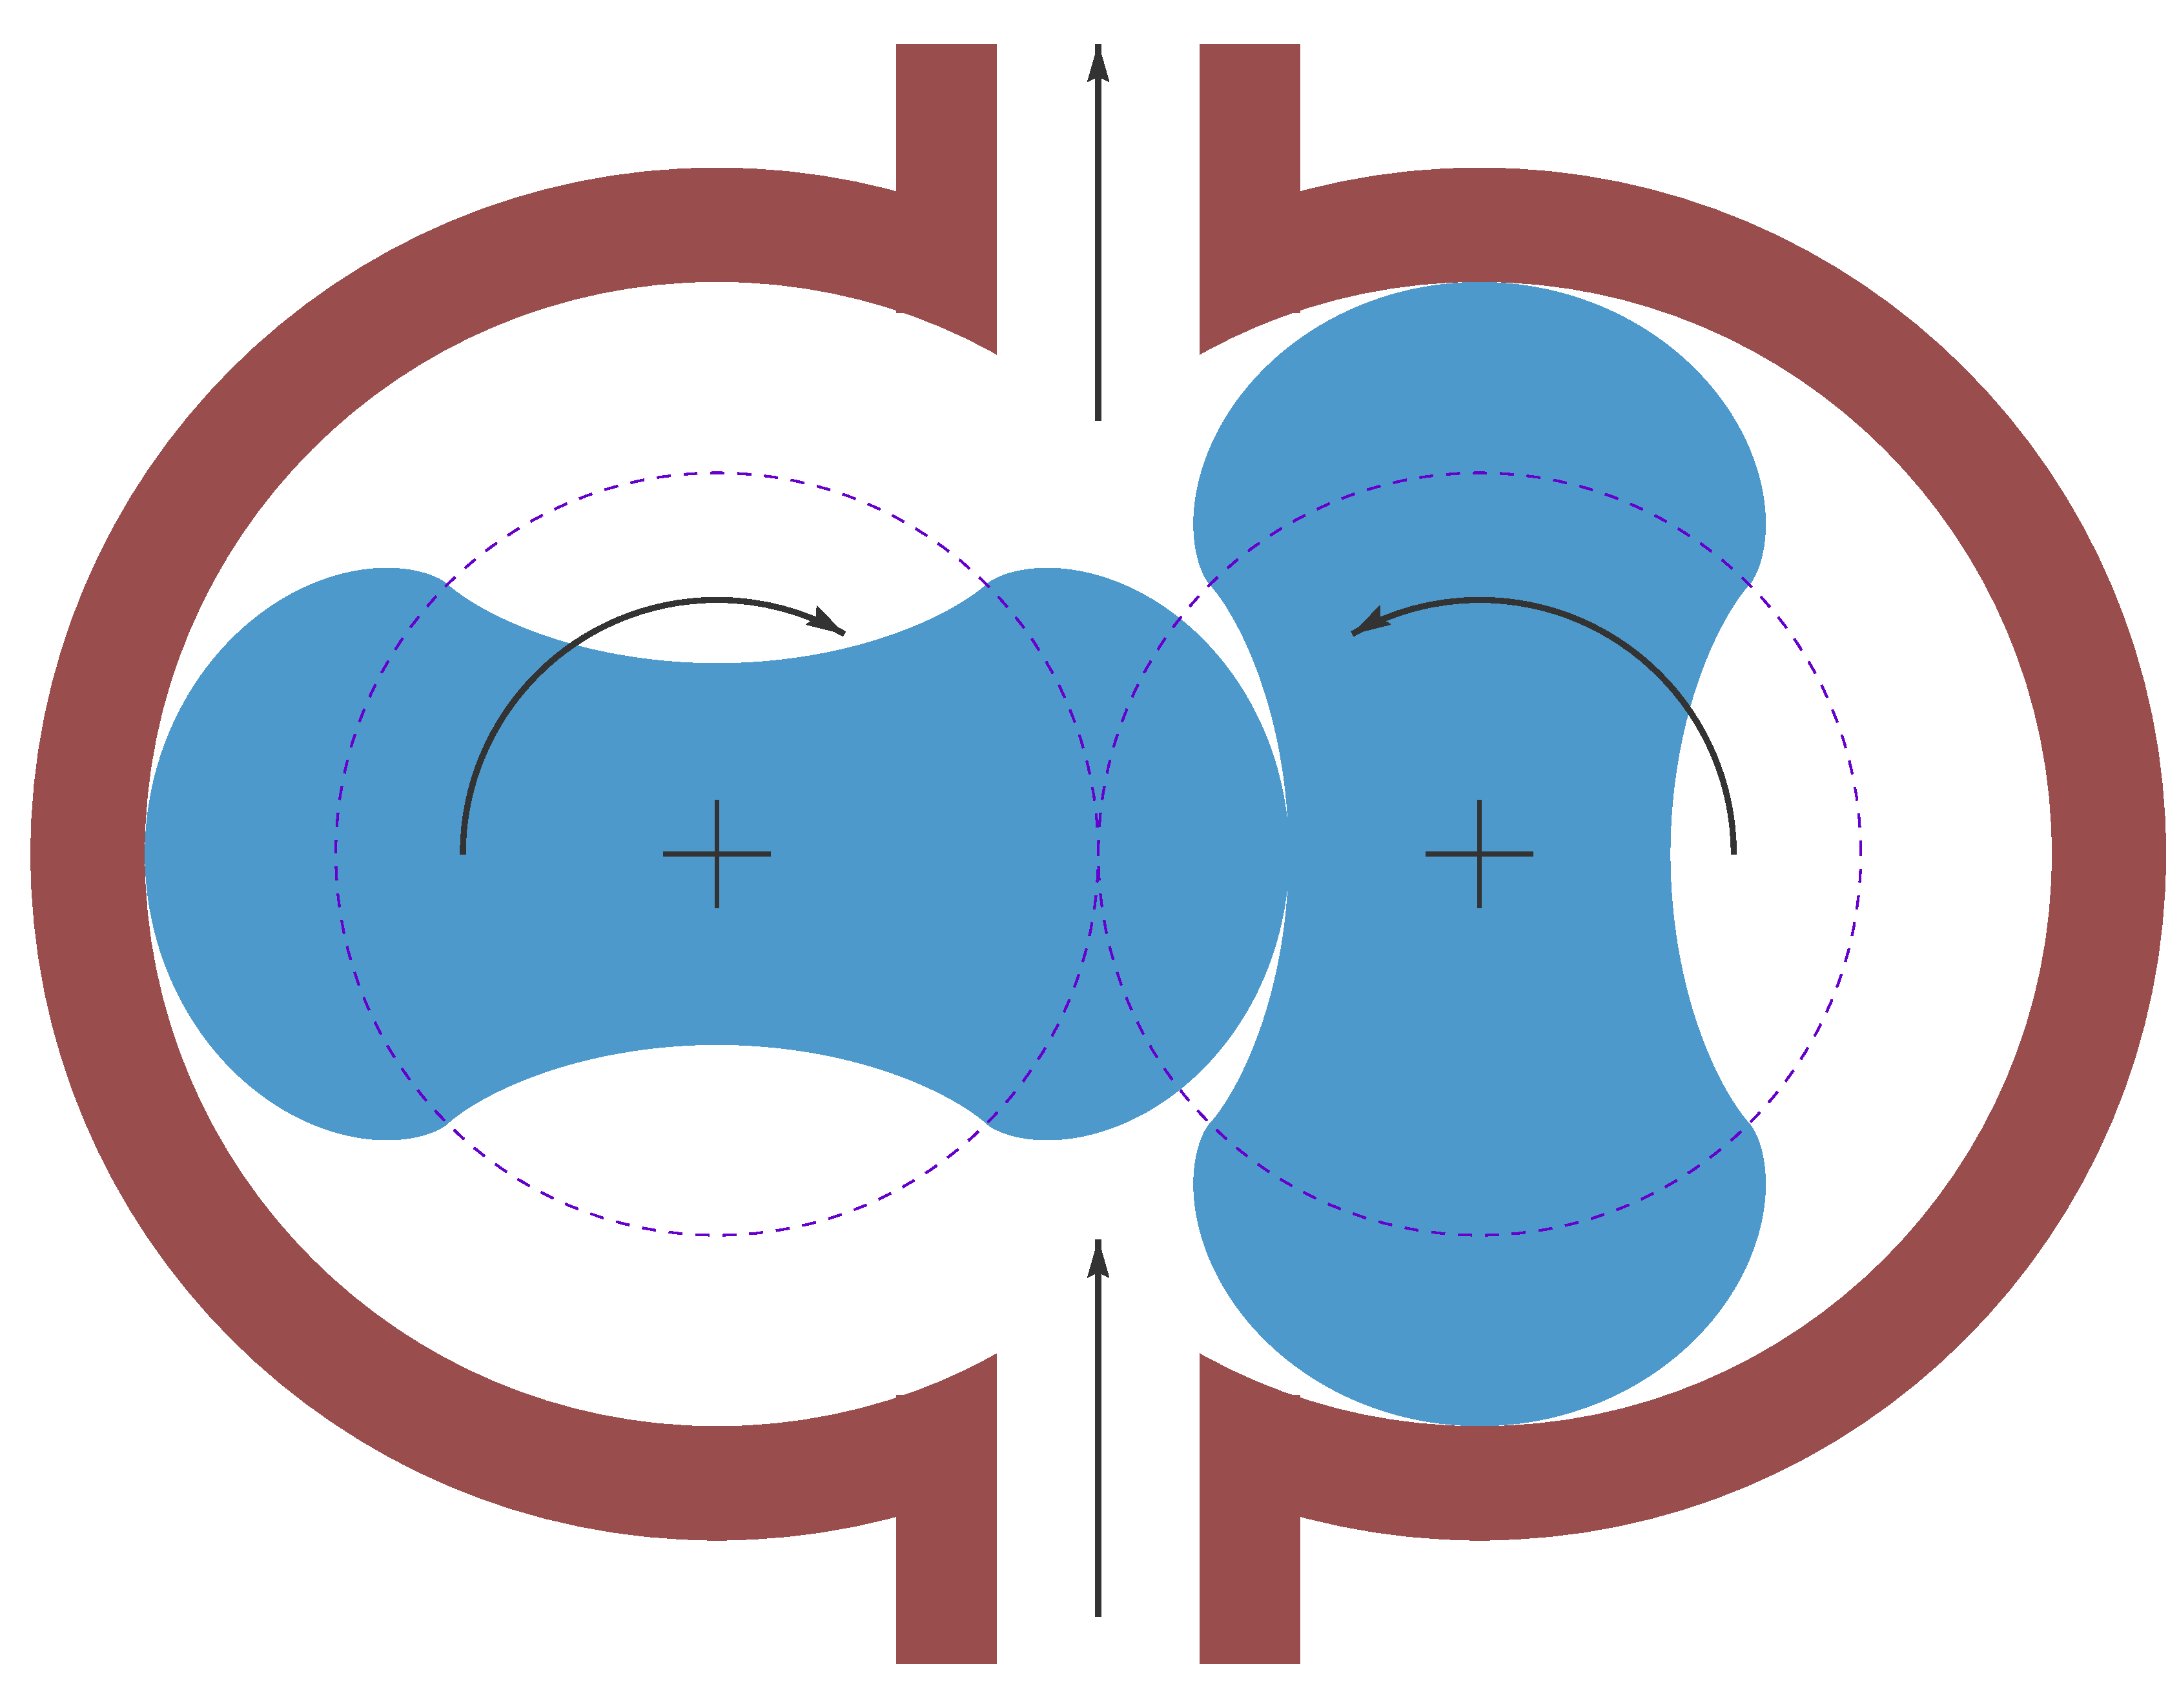
\includegraphics[width=0.9\textwidth]{part3/ruote/FIG/ruote/kompressor.pdf}
     \end{center}
\begin{picture}(0,0)(0,0)
        \scriptsize{
        \put(245,143){$O_1$}
        \put(130,143){$O_2$}
        \put(245,195){$\omega$}
        \put(130,195){$\omega$}
	\put(171,230){\rotatebox{90}{Uscita}}
	\put(171,50){\rotatebox{90}{Ingresso}}
}
\end{picture}
\vskip -5mm
        \caption{
\em Compressore a lobi ottenuto dall'ingranaggio di due ruote cicloidali a due denti.
}
     \label{fig:kompressor}
\end{figure}

\noindent Vi \`e un ambito della meccanica, molto particolare,
 dove le ruote cicloidali
la fanno da padrone, ed \`e quello dei {\em meccanismi per orologeria}\index{ruote!per orologeria}.
Si tratta, come \`e facile intuire,
 di un mondo piuttosto distante da quello della meccanica delle
macchine. L'ingombro delle ruote dentate per orologeria deve essere
infatti compatibile con le dimensioni degli orologi che le ospitano,
 quindi il loro diametro
spesso non supera i 10--15 millimetri. Altre
caratteristiche
salienti di questo speciale settore degli ingranaggi sono l'assenza sistematica
di lubrificazione e i valori minuscoli dei flussi di potenza, flussi che, non
presentando mai inversioni di direzione, rendono tollerabili (quando
non prescritti) giochi rilevanti tra le dentature.
Una volta scritta la procedura numerica
dalla quale otteniamo le figure \ref{fig:1160cy} e \ref{fig:kompressor},
la curiosit\`a di vedere tale codice all'opera
con le ruote per orologeria era elevata. La 
fortuna e la casualit\`a ci hanno fatto imbattere in un testo che potrebbe
aver rappresentato per un bel po' di tempo il riferimento degli orologiai: 
\cite{grossmann}. Per la verit\`a il libro ora citato, nell'opportuno
capitolo dedicato agli ingranaggi, considera anche le ruote con profilo
ad evolvente. Ma \`e subito abbastanza chiaro che lo fa per completezza, e che
le ruote a profilo cicloidale saranno al centro di tutte le successive
considerazioni. Siamo certi che la norma \cite{bs978}, la quale propone
una standardizzazione delle ruote per orologeria, sia stata, in larga parte,
elaborata seguendo \cite{grossmann}.
Nel paragrafo \ref{percorso-ruote}
tra i precetti che abbiamo messo in campo, nel nostro percorso intuitivo,
ve ne era uno, debole, il quale prescriveva che ci fosse una sola famiglia di 
ruote di assortimento, e non due. Ma tale precetto veniva appunto 
etichettato 
come debole, anzi, in quello stesso luogo indicavamo questo capitolo
di approfondimento come la sede
dove si descrive una serie di ingranaggi formata da due famiglie 
diverse di ruote.
In orologeria, di fatto, pignoni e ruote non possono essere confusi tra loro
e l'ingranamento pignone-pignone o ruota-ruota non \`e mai 
possibile. Addirittura,
la nomenclatura delle loro sporgenze \`e eterogenea: i pignoni ospitano
le foglie, le ruote i denti. Queste due famiglie di ruote dentate nascono
dalla volont\`a di ottenere, sia per i pignoni, sia per le ruote,
denti il cui
profilo risulti il pi\`u 
semplice possibile da tagliare. Per questo motivo, si fa in modo di utilizzare
sia sul pignone sia sulla ruota un ipociclo di raggio esattamente pari
alla met\`a
del loro raggio primitivo. L'ipocicloide cos\`i ottenuta coincide con un
diametro della primitiva, pertanto si presenta rettilineo e radiale.
\begin{figure}[b]
     \begin{center}
     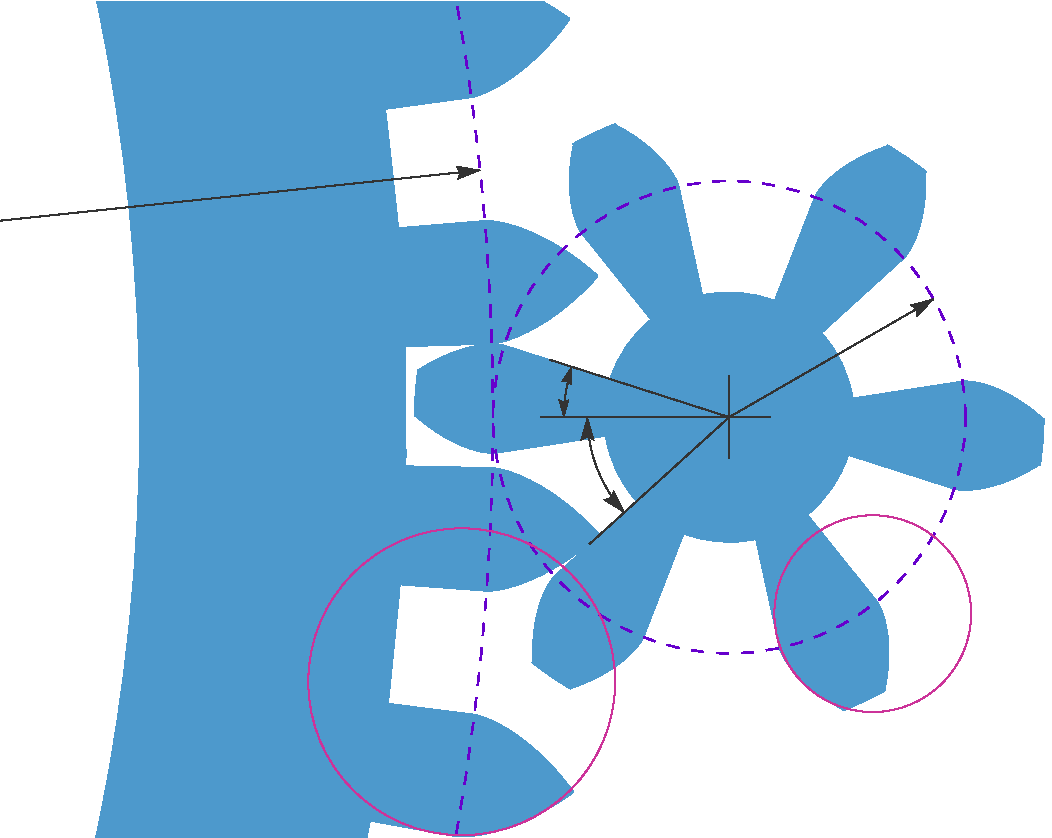
\includegraphics[width=0.9\textwidth]{part3/ruote/FIG/ruote/660cy_hor.pdf}
     \end{center}
\begin{picture}(0,0)(0,0)
        \scriptsize{
        \put(150,222){$r_2$}
        \put(288,189){$r_1$}
        \put(180,162){$\alpha_a$}
        \put(193,136){$\alpha_r$}
        \put(245,145){$O_1$}
        \put(205,50){$r_{e_2}=1.949 m$}
        \put(207,40){BS 978-2}
        \put(290,59){$r_{e_1}=1.25 m$}
        \put(290,49){BS 978-2}
}
\end{picture}
\vskip -5mm
        \caption{
\em Ingranaggio cicloidale da orologeria, pignone con $z_1=6$ foglie, ruota
da $z_2=60$ denti. Accesso $\alpha_a=17^{\circ}44'$, recesso $\alpha_r=42^{\circ}16'$.
}
     \label{fig:660cy_hor}
\end{figure}
Ovviamente le epicicloidi, che costituiranno il profilo delle
teste dei denti, saranno ottenute dalle stesse rollette, gi\`a utilizzate
per gli ipocicli, a primitiva invertita.
La figura \ref{fig:660cy_hor} riporta un ingranaggio con $z_1=6$ e $z_2=60$
in cui risultano evidenti i fianchi rettilinei delle foglie del
pignone  e dei denti della ruota.
Non \`e difficile comprendere che i fianchi rettilinei dei denti
risultano di facile lavorazione, potendo essere tagliati da sottili 
fese a disco con taglienti piani. In altre parole non \`e necessario che la
sezione della fresa abbia la forma del vuoto tra i denti.
Sembra che gli appassionati di questo settore riescano a tagliare queste
minuscole ruote persino con utensili pi\`u o meno hobbistici,
 certamente aiutati
da opportuni apparecchi divisori. Le teste ({\em addendum}) delle foglie
del  pignone e dei denti della ruota meritano invece considerazioni
distinte. Cominciamo con l'osservare che i rapporti di trasmissione
utili in orologeria sono una manciata. In \cite{grossmann} ne sono
specificati sedici e l'autore dice esplicitamente di averne riportati
pi\`u di quelli realmente in uso. Le moltipliche che si eseguono
sono ancor meno delle coppie trattate, ad esempio la moltiplica per
dieci si pu\`o ottenere con gli ingranaggi
 60--6, 70--7 e 80--8. Parliamo di moltiplica
perch\'e, in generale, in quest'ambito, sono le ruote a muovere i pignoni. 
Da quest'ultima considerazione, dal fatto cio\`e che siano
le ruote ad essere motrici, si identificano naturalmente il
tratto di accesso e quello di recesso, i quali si toccano sulla
linea immaginaria che congiunge il centro della ruota a quello del
pignone.
Nel paragrafo \ref{ruote-corr1} abbiamo accennato alla dissimmetria
di cui soffrono accesso e recesso rispetto al rendimento dell'ingranaggio:
durante il recesso, il rendimento \`e sempre pi\`u elevato.
In un ambito dove la ridottissima quantit\`a di energia disponibile proviene da
una molla, o da un peso che scende, oppure da una piccola batteria, e
tale energia deve muovere il meccanismo dell'orologio il pi\`u a lungo
possibile, risulta quindi naturale 
la tendenza ad avere il minimo arco di accesso e il massimo
arco di recesso, compatibili con la geometria delle ruote coinvolte.
L'angolo di recesso maggiormente esteso
si ottiene con la massima altezza realizzabile per i denti della ruota.
Il profilo dei denti viene pertanto esteso fino ad appuntire il dente
stesso. L'ultima posizione utile del dente nel recesso si ha quando la
tangente sulla punta dell'{\em addendum} \`e parallela al fianco rettilineo della
foglia, come mostrato in figura.
Nella pratica costruttiva di queste ruote, tali fianchi che,
teoricamente, dovrebbero essere epicicloidali,
 vengono approssimati da archi di circonferenza,
facili da improntare direttamente sulla fresa a disco che taglia la
ruota.  Lo {\em standard}
 B.S. 978, \cite{bs978}, che raccoglie in compendio le raccomandazioni
di una vasta parte dell'industria svizzera di orologi, raccomanda di sostituire
la porzione epicicloidale del fianco del dente con un arco di circonferenza di
raggio medio rispetto all'epicicloide stessa. Mentre in \cite{grossmann}
il proporzionamento delle ruote e dei pignoni avviene con riferimento
al loro diametro e al  loro numero di denti, nelle raccomandazioni raccolte
in \cite{bs978}, immaginiamo
con l'intento di dare maggiore sistematicit\`a ai parametri che regolano
la geometria di queste ruote, si parte da una tabella di moduli, in mm, 
dove su circa sessanta valori standardizzati, spiccano in grassetto
0.08, 0.1, 0.15, 0.2, 0.25, 0.3, 0.4, 0.5, 0.6, 0.7, 0.8, 1.0.
Giusto per rendere l'idea del perimetro entro il quale ci muoviamo,
una ruota con 60 denti e modulo 0.1 mm avr\`a un diametro primitivo pari
a 6 mm. Parlando dei denti delle ruote, sempre in \cite{bs978}, si trova
la tabella 2 che lega i loro dettagli geometrici,
 come {\em addendum}, {\em dedendum},
raggio e posizione del centro dell'arco di circonferenza che sostituisce
lo spezzone di epicicloide e spessore del dente, al modulo
della ruota stessa.
Alcune di queste dimensioni, in particolare il raggio dell'arco
di circonferenza che costituir\`a l'{\em addendum}, dipendono per\`o, oltre che dal
modulo, anche dal rapporto di trasmissione e dal numero di foglie del
pignone col quale la ruota \`e destinata a ingranare.
Fortunatamente, come abbiamo gi\`a accennato,
sia i rapporti di trasmissione, sia i numeri delle foglie che si usano
sono limitati. Per questo motivo risulta agevole
costruire la tabella 3 di \cite{bs978},
che riporta per nove numeri delle foglie del pignone, da 6 a 16 saltando 11 e 13,
e per 14 valori del rapporto di trasmissione, i valori che identificano
geometricamente il dente della ruota in questione.
Nella nostra figura \ref{fig:660cy_hor}, la ruota ha sessanta denti mentre
il pignone presenta sei foglie, e abbiamo lasciato, sia per l'{\em addendum}
della ruota, sia per quello del pignone, i tratti di epicicloide calcolati.
\begin{figure}[b]
     \begin{center}
     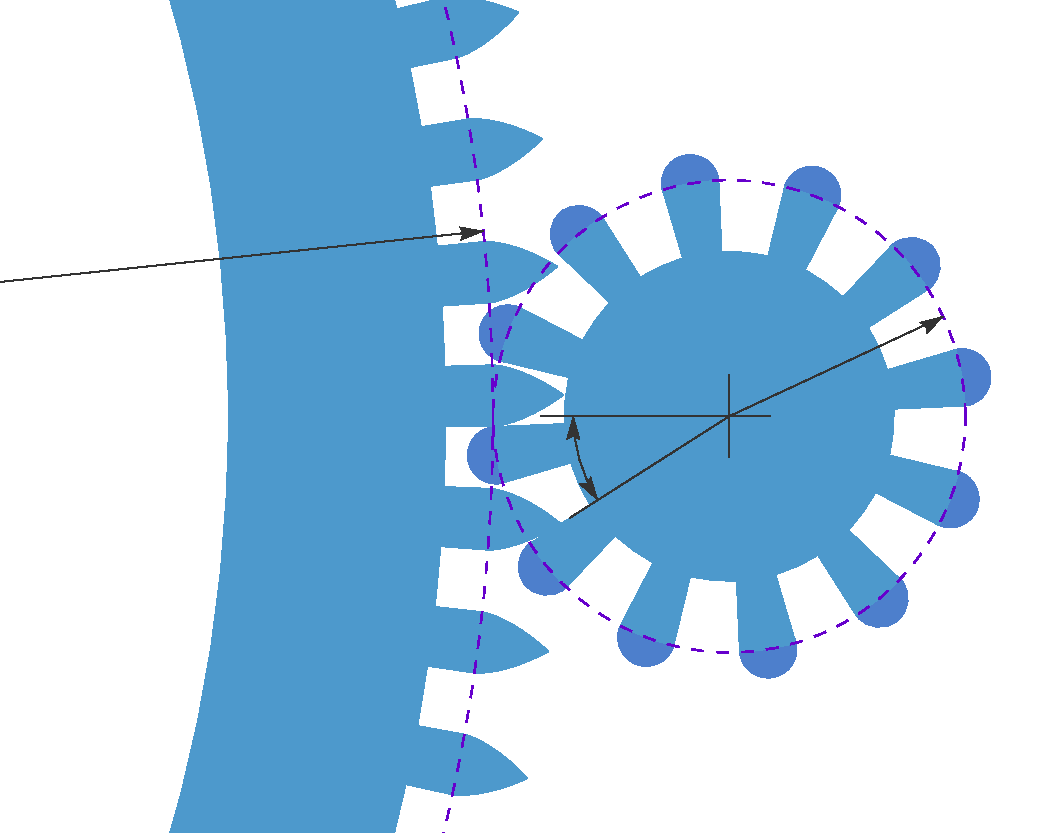
\includegraphics[width=0.9\textwidth]{part3/ruote/FIG/ruote/1290cy_hor.pdf}
     \end{center}
\begin{picture}(0,0)(0,0)
        \scriptsize{
        \put(156,215){$r_2$}
        \put(295,184){$r_1$}
        \put(187,134){$\alpha_r$}
        \put(245,145){$O_1$}
}
\end{picture}
\vskip -5mm
        \caption{
\em Ingranaggio cicloidale da orologeria, pignone con $z_1=12$ foglie, ruota
da $z_2=90$ denti. Ingranaggio a tutto recesso $\alpha_r=32.5^{\circ}$.
}
     \label{fig:1290cy_hor}
\end{figure}
Riportiamo comunque in figura anche le circonferenze
approssimanti indicate in \cite{bs978}, in modo da avere un riscontro visivo
circa la loro effettiva bont\`a. 
Una volta calcolato, tramite
la nostra procedura numerica, oppure consultando \cite{grossmann}, pag. 175,
il massimo angolo di recesso, $\alpha_r$,
dobbiamo garantire un angolo di accesso che sia $\alpha_a> 2 \pi/z_1 -\alpha_r$,
in modo da poter assicurare la continuit\`a della trasmissione.
Nel nostro caso abbiamo
un recesso molto pi\`u esteso dell'accesso. L'epicicloide dell'{\em addendum}
delle foglie del pignone sar\`a pertanto impegnata in un suo breve tratto
vicino alla circonferenza primitiva. Per questo motivo l'approssimazione
del tratto di epicicloide sulle foglie dei pignoni \`e ancora pi\`u facile
di quella che si esegue sui denti delle ruote.
Tanto \`e vero che in molti casi, come quello che riportiamo in figura
\ref{fig:1290cy_hor}, l'{\em addendum} sulle foglie non lavora. Per tale ingranaggio
l'arco di accesso \`e nullo e l'arco di recesso vale $\alpha=32.5$, 
gi\`a superiore ai necessari $30^{\circ}$. La sommit\`a delle foglie presenta quindi
arrotondamenti senza alcuna funzione cinematica, ma che rendono i pignoni
maggiormente compatibili con l'ingranamento: non sarebbero apprezzabili
gli spigoli vivi sulla cima delle foglie, qualora fossero terminate
alla fine dell'ipociclo rettilineo. Tali arrotondamenti oziosi
vengono messi in evidenza, in colore pi\`u scuro,
nella stessa figura.
In entrambe le figure, \ref{fig:660cy_hor} e \ref{fig:1290cy_hor}, si pu\`o
notare un gioco notevole tra le dentature, funzionale alla
robustezza dell'ingranaggio nei confronti della possibile
intrusione di corpi estranei (polvere), il cui valore \`e
stato determinato seguendo le raccomandazioni di \cite{bs978}.
Come gi\`a accennato altrove, tale gioco non suscita inconvenienti, in quanto
la potenza trasmessa \`e minuscola e oltretutto, in generale, il
suo flusso non presenta inversioni.
\endinput
